\newcommand{\genf}{ {\textsf {f}} }
%\newcommand{\fbar}{\underline{f}}
\newcommand{\dbar}{\underline{\d}}
\newcommand{\Fbar}{\underline{F}}
\newcommand{\fbar}{\underline{f}}
%\newcommand{\adjoint}[1]{\bar{#1}}
\newcommand{\fadj}{\adjoint{f}}
\newcommand{\Fadj}{\adjoint{F}}
\newcommand{\radj}{{\adjoint r}}
\newcommand{\psidot}{\dot{\psi}}
\renewcommand{\star}{\ast}
%\newcommand{\dprime}{{\prime\prime}}
\renewcommand{\C}{{\cal C}}
\renewcommand{\L}{{\cal L}}

\chapter{An Introduction to Geometric Calculus 70\%}\label{ch:gc}

\section{Introduction}

%The usefulness of vector algebra in physics does not need much advocating.
%Early in our eductation we learn the scalar and vector products,
%Stokes theorem and Gauss' divergance theorem.
%With these many of the laws of classical mechanics are written consisely in a
%frame independant way. 
%With the frame independance comes clarity,
%the relations encoded in the mathematics describe the relations observed in the
%world.

%But this eligance is soon lost:
%the vector product is defined only in three dimensions.
%In  two dimensions, where complex analysis and Cauchy's
%theorem are so useful, there is nowhere for the `axial' vector of the
%cross product to go.  
%Likewise in the four dimensions of relativistic physics,  
%there are an infinate number of axial vectors to a plain.
%The abstract vector algebra that had been used so profitably is abandoned in favour of
%components in some chosen basis.
%And worse still is the confusion that can arrise as to what 
%purpose a particular coordinate frame serves.
%Is it to compensate for a lack of an adiquate vector algebra in four
%dimenstions,
%or is it to describe how phsysics appears to a particular observer?
%As \cite{Doran2003} note:
%\begin{quote}
%  From a study of the literature on relativity one can easily form the
%  impression that the subject is in the main concerned with
%  traformations betweeen frames. But it is the subject of relativistic
%  dynamics that is of primary importance...
%\end{quote}
%But this is just the beginning of our troubles.
%When written in terms of co-ordinates there are subtables in the  very notion of a
%transormation itself!
%\cite{Hestenes1984} put it like this,
%\begin{quote}
%  Covariant tensor analysis makes it difficult to distinguish between
%  a tensor's behavior under transformations and its linear properties.
%  A distinction between {\em active} and {\em passive} transformations
%  is commonly made.  It is important to note that the covariant
%  formalism itself provides no means to represent the distinction.
%  The equations for both types of transformation are identical, and
%  the distinction is made only in the interpretations of the
%  equations. Textbooks are littered with evidence of muddles that
%  arise from this practice.
%\end{quote}

%Much of the difficulty of modern physics lies in the lack of clarity
%in its mathematical exression.
%The introduction of auxillary fields to maintain local gauge
%invariance rapidly leads to a sea of indices.
%And similarly if curved  geometries are considered,
%then once again we  drown in an index soup.
%Our equations fall victim to a proliferatoin of
%book-keeping devices such as Christoffel connections that maintain a
%cooridinate basis that may or may not reflect the symmetries in the problem. 
%Trying to hold onto a feeling for what any given relation is expressing soon
%becomes a fight with its representation that not many win.


%And we can most certainly do better.
%The \GC\ developed by David Hestenes in the 1960s overcomes all of the
%above frailaties in representation discussed above.
%With the introduction of a new product,
%the geometric product, 
%that links the scalar product and Grassman's exterior products,
%comes the generalisation of complex variable theory and the vector
%product to arbitary dimensions.
%With this comes the unification of Cauchy's integral theorem, Stokes
%theorem and the divergance theorem as special cases of a single
%integral formula.
%Further, as one would expect with the generalisation of complex
%variable theory,
%rotations are handled with exceptional efficiancy.
%This has many applications.

% \GC\ has a very useful specialisation, space-time algebra (STA) that
% encodes the physics on a Minkowski signature with great efficientcy,
% in addition to providing a very clear and elegant method of splitting
% the results into different relative frames for particular observers.
% This enables all of Maxwells relations to be expressed in a single
% equation, something not possible with convensional formualtions that
% don't link the scalar and exterior product.
% \GC\ simplifies and clarifies the representation of quantum theory.
% Principle among its successes is the expression of the Dirac equation
% in terms of a real algebra with 8 independant parameters,
% cutting in half the number of the conventional representation
% and thereby removing a great deal of redunancy of notation.
% The geometrical interpretation facilitated by such a representation
% also brings to the fore the links that can be made to the classical
% world.
% For example, both Pauli algebra and spinors have a clear geometrical significance that
% is very helpful to classical as well as quantum problems.

%To introduce \GC\ adiquatly would require a books worth of space.
%And since such books have already been written, 
%with \cite{Hestenes1984} describing the mathematics in detail, 
%and \cite{HestenesMechanicsBook} and \cite{Doran2003} describing the application of
%\GC\ to physics, a full introduction to \GC\ will not be attempted here.
%However, to keep the report self contained,
%a short introduction to the algebra will be given.
%None of the results in this chapter are new.
%Most have come from \cite{Hestenes1984}, 
%often  written there with greater generality than here.

%Before the algebra is introduced formally, however,
%we begin with an example that illustrates the basic approach,
%and brings to the fore some of the similarites of geometry to complex
%algebra.






The section on functional differentiation follows the exposition of \cite{AltlandBook, Doran2003} and
\cite{ FramptonBook}.

\section{Geometric Algebra}


\begin{figure}%[htp]
 \centering
 \includegraphics{lattice.3}
 \caption{
   A lattice depicting the relationship between scalars, vectors, areas and volumes in three dimensional space.
}
 \label{fig:lattice_3D}
\end{figure}


An $n$-dimensional geometric space can be parameterised by a frame of orthonormal vectors, $\{e_1,e_2,\ldots, e_n\}$.
From these, a set of $\nCr{n}{2} \equiv n(n-1)/2$ independent area elements can be constructed,
 a set of $\nCr{n}{3}$ volume elements,
and so on up to a single $n$-dimensional hyper-volume.
The relationship between these $2^n$ elements can be drawn in a Hesse-diagram,
and the case for three dimensions is drawn in \figref{lattice_3D}.

The word {\em grade} is used to describe the different levels of the lattice drawn in \figref{lattice_3D}.
So the scalar values at the base of the lattice are grade 0.
The vector elements are grade 1, the area elements grade 2, and so on.
Referring to the top element as the ``grade-$n$ hyper-volume in an n-dimensional space'' is cumbersome.
Rather, the symmetry of the lattice is invoked and the top element is referred to as the {\em pseudoscalar}. 
It is denoted with the symbol $I$.
Likewise, the elements that are of grade $n-1$ can be referred to as the {\em pseudovectors}, although this terminology is used less often.

To be able to describe such geometrical entities mathematically, 
we need an algebra that is able to navigate through lattices such as the one drawn in \figref{lattice_3D}.
David Hestenes developed the mathematics to do so midway through the twentieth century,
by extending and generalising the geometric machinery of Hilbert, Clifford and Grassmann.
The resulting algebra is called {\em Geometric Algebra}.


\begin{figure}%[htp]
 \centering
\missingfigure{The interpretation of the outer product between vectors}
 \caption{
   Geometric interpretation of the outer product.
   Between the vectors $a$ and $b$,
   the outer product defines an orientated area of magnitude $\abs{a}\abs{b}\sin(\theta)$.
}
 \label{fig:outer_product}
\end{figure}

\subsection{The outer-product}

Grassmann's exterior product is what is required to the join geometric elements together and climb the lattice.
The product is denoted with a wedge, $\wedge$, and in Geometric Algebra is referred to more simply as the {\em outer product}.
The area $e_1\wedge e_2$, for example, denotes the area element created from the vector $e_1$, first, and then the vector $e_2$.
The ordering in which the area is constructed gives an orientation to the area element,
which is reversed if the order in which the area is constructed is reversed.
Therefore we have,
\begin{align}
  e_1 \wedge e_2 = -e_2 \wedge e_1
\end{align}
from which it follows that the outer product is anti-commutative and that $a \wedge a = 0$ for any vector $a$.
Between two arbitrary vectors, $a$ and $b$, the outer product defines the area swept out by the vectors.
Its magnitude is $\abs{a}\abs{b}\sin(\theta)$,
where $\theta$ is the angle between the vectors.
The geometric interpretation is illustrated in \figref{outer_product}.
Volumes can be similarly constructed,
and so in three dimensions the pseudoscalar is 
\begin{align}
  I = e_1\wedge e_2 \wedge e_3 = - e_1\wedge e_3 \wedge e_2 =  e_3 \wedge e_1 \wedge e_2  = - e_3 \wedge e_2 \wedge e_1.
\end{align}
It is to be emphasised that the pseudoscalar gives an {\em orientated} volume element.

\subsection{The inner-product}

Next, we need to be able to descend down the lattice of geometric elements.
This is achieved with the {\em inner-product}, which is denoted with a central dot, $\cdot$.
The inner product defines the subspace remaining when two geometric elements are projected onto each other.
For example, the inner-product between the vector $e_1$ and the volume $e_1\wedge e_2 \wedge e_3$
is the area $e_2\wedge e_3$.
For the vectors $e_1$ and $e_2$ the inner product is zero:
between orthogonal vectors there is no subspace remaining after the projection.
For two arbitrary vectors, $a$ and $b$, the inner product gives a scalar length of the shared subspace,
\begin{align}
  a\cdot b = \abs{a}\abs{b}\cos(\theta).
\end{align}
In general, for arbitrary vectors, $a$, $b$ and $c$, and scalar $\lambda$,
the inner-product satisfies
\begin{align}
  \lambda \cdot a &= 0 \\
  a\cdot b &= b\cdot a\\
  a\cdot(\lambda b) &= \lambda \lr{a\cdot b}\\
  a\cdot(b+c) &= a\cdot b + a\cdot c.
\end{align}

More generally, the inner-product between an arbitrary vector $a$ and higher grade elements is given by
\begin{align}
  a \cdot \lr{a_1\wedge a_2 \wedge\ldots \wedge a_r} = 
  \sum_{k=1}^r (-1)^{k+1} a\cdot a_k a_1 \wedge \ldots \wedge \check{a}_k
  \wedge \ldots \wedge a_r,
 \label{eqn:dot_multiwedge}
\end{align}
where the check denotes that the vector is missing from the product.
We refer to Hestenes\cite{Hestenes1984} for the proof.
Equation \eqnref{dot_multiwedge}
has the useful special case,
\begin{align}
 a\cdot (b \wedge c) = a \cdot b c - a\cdot c b.
 \label{eqn:dot_wedge}
\end{align}

\subsection{The geometric product}

One final product is needed to complete this introduction to geometric algebra,
and that is the {\em geometric product}:
\eqal{
 ab &= a\cdot b + a\wedge b. %\\
 %&= \scalar{ab} + \bi{ab} \\
%    &= \frac{ab + ba}{2} 
}{geometric_product}
The geometric product is a {\em mixed grade} product,
it results in geometric entities that are both of lower and higher grade than the elements that participate in the product.

The introduction of the geometric product means that we need a convention on the ordering of products.  In the absence of parenthesis, the inner or outer product are always evaluated before the geometric product.  Equation \eqnref{dot_wedge} demonstrates this convention. 


From the respective commutivity and anti-commutivity of the inner and outer product,
it follows that for vectors $a$ and $b$, 
\sub{
\begin{align}
a\cdot b &=\frac{ab+ba}{2}\\
a\wedge b &=\frac{ab-ba}{2}.
\end{align}
\label{eqn:dot_wedge_product}
}
If $A_r$ is a multi-vector of grade $r$ then \eqnref{dot_wedge_product}
can be generalised to
\sub{
\begin{align}
a \cdot A_r &= \multi{a A_r}{r-1} = \frac{a A_r- (-1)^r A_ra}{2}\\
a\wedge A_r &=\multi{a A_r}{r+1} = \frac{a A_r + (-1)^r A_ra}{2}.
\end{align}
\label{eqn:dot_wedge_product_gen}
}
so that
\begin{align}
a A_r =  \multi{a A_r}{r-1} + \multi{a A_r}{r+1} = a \cdot A_r + a\wedge A_r.
\label{eqn:gp_vect_multi}
\end{align}
In equations \eqnref{dot_wedge_product_gen} and \eqnref{gp_vect_multi}
we have introduced the grade operator, $\multi{\ldots}{r}$, to denote the $r$-vector part of the bracketed quantity.  
%of only a particular grade of a geometric quantity: $\multi{a A_r}{r-1}$ denotes the part of the geometric product between $a$ and $A_r$ that results in an entity that is of grade $r-1$.
This notation helps to emphasise that the inner-product  lowers the grade, 
and the outer-product raises the grade.
For convenience we omit the subscript zero on scalar quantities,
so that $\multi{ab}{0} \equiv \scalar{ab}$.
Again, we refer to Hestenes\cite{Hestenes1984} for the proof of \eqnref{dot_wedge_product_gen}.

The usefulness of the geometric product can be powerfully illustrated in two dimensions.
Introducing the orthonormal frame $\{e_1,e_2\}$,
the pseudoscalar is the area element $I= e_1\wedge e_2 = e_1 e_2$.
By first noting that 
\begin{align}
I^2 = e_1e_2e_1e_2 = -e_1e_2e_2e_1 = -1,
\end{align}
and then decomposing the arbitrary vector $a$ in terms of the basis,
\begin{align}
 a  = \abs{a}\cos(\theta)e_1 + \abs{a}\sin(\theta)e_2
\end{align}
it is easy to see that the geometric product of $e_1$  with  $a$ results in
\begin{align}
   e_1a  =  e_1\cdot a + e_1\wedge a = \abs{a}\lr{\cos(\theta) + I \sin(\theta)} =  \abs{a} e^{I\theta}.
\label{eqn:deMorgan}
\end{align}
It can be immediately seen that equation \eqnref{deMorgan} is the de Morgan decomposition of a complex number,
with the pseudoscalar $I$ taking the role of the `complex scalar'.

Furthermore, we notice further that due to the anti-commuting properties of the outer-product,
\begin{align}
  a e_1  =   \abs{a}\lr{\cos(\theta) - I \sin(\theta)} =  \abs{a} e^{-I\theta}.
\label{eqn:deMorgan_conj}
\end{align}
In the language of complex variables, $e_1 a$ and $a e_1$ are conjugate to each other.
This encourages the definition of the {\em reverse} operator, which will be denoted with a dagger,
\begin{align}
  \lr{a_1 a_2 a_3 \ldots a_r}^\dagger = a_r a_{r-1} \ldots a_1.
\end{align}
Therefore, if $z \equiv e_1 a = \abs{a} e^{I\theta}$ then $z^\dagger = \abs{a} e^{-I\theta}$.

\subsection{Reflections and rotations}

The next examples of the power of the geometric product come from the ease at which simple geometric operations may be expressed.
First we consider the reflection of a vector $a$ in the (hyper)plane that is perpedicular the unit-vector $n$.
To do so, we evaluate the components of the vector that are parallel and perpendicular to $n$, $a_{\parallel}$ and $a_\perp$, respectively,
%and the component that is orthogonal to the plane $a_\perp$,
\begin{align}
a &= n^2 a \\
  &= n \lr{n\cdot a + n\wedge a}\\
  &= a_\parallel + a_\perp.
\end{align}
That is,
\begin{align}
  a_\parallel &= n n\cdot a & a_\perp &= n n\wedge a.
\end{align}
The reflection in the plane is then, simply,
\begin{align}
  a^\prime &= a_\perp - a_\parallel \\
  &= -n \lr{a \wedge n + a\cdot n}\\
  &= -nan.
\label{eqn:reflection}
\end{align}
No reference was made to the dimension of the space when deriving equation \eqnref{reflection}.
It is an entirely general formula.

Rotations can be handled similarly.
This is because a rotation in a plane that is generated by unit vectors $m$ and $n$ is generated 
by two reflections in the (hyper)planes perpendicular to $m$ and $n$.
The angle of the rotation is twice the angle between the vectors $m$ and $n$\todo{Some evidence for this will be nice}.
That is, by applying equation \eqnref{reflection} twice,
\begin{align}
a^\prime = nmamn
\end{align}
represents a rotation of the vector $a$ in the plane defined by $m\wedge n$ by an angle $2\phi$, 
where $\phi$ is the angle between $m$ and $n$.

The product $mn$ therefore represents a rotation operator,
$R = mn$,
so that a rotation of a vector, $a$, through an angle $\theta$ may be defined
\begin{align}
  {\cal R}\lr(a, \theta) = RaR^\dagger = e^{I \theta/2}ae^{-I \theta/2}
  \label{eqn:rotation}
\end{align}
where $I$ is the unit area element through which the rotation occurs.
Again, equation \eqnref{rotation} is independent of the dimension of the space.

The polar form of the complex variable can now be understood.
By noting that 
\begin{align}
  e_1  e^{I\theta} =  e^{-I\theta}e_1 =  e^{I\theta/2}e_1  e^{-I\theta/2}
  \label{eqn:complex_triplet}
\end{align}
we see that the polar form represents a rotation through the complex plain.
This conforms to the standard interpretation.
However,
we can now understand the form given in equation \eqnref{deMorgan} 
to be a special case of the general rotation formulat given in equation \eqnref{rotation}.
The equality of the three forms given in \eqnref{complex_triplet} result 
only because the vector $e_1$ is in the same plane as the plane of rotation.
This does not generally follow.
Equation \eqnref{rotation} gives the general result.

\section{Set and Lattice Theory}

The three products of geometric algebra form the basis of a very power algebra.
It will be useful to absorb other useful algebras into this framework,
so that we have a single powerful approach rather than many weaker tools.
In this section, we frame the operations of set and lattice theory in Geometric algebra.

\subsection{The dual of a vector space}.

The first operation that is required is that of duality.
The dual of a geometric entity is the subspace that encompasses everything apart from the given entity,
so that taken together, the whole space is spanned.

The join of two


The pseudoscalar makes the dual easy to define.
For the multivector $A$ it is 
\begin{align}
  \tilde{A} \equiv A I^\dagger.
\end{align}
If $A$ is not a scalar than this reduces to $ \tilde{A} = A \cdot I^\dagger$.
The double dual is 
\begin{align}
  \lr{\tilde{A}}\tilde{} = (-1)^{n(n-1)/2} A.
\end{align}

The meet of two geometric entities is the maximal subspace that is shared by both entities.
Th intersection.
It can be determined by duality,
\begin{align}
  A \meet B \equiv \lr{\tilde{A}\wedge \tilde{B}}\cdot I
\end{align}
so that
\begin{align}
  \lr{A\meet B}\tilde{} = \tilde{A}\wedge\tilde{B}.
\end{align}
Note that the meet and the join are orientated.



% The de Morgan representation of a complex number admits the geometrical interpretation of a rotation operator.
% A vector along the real number line (taken here to be $e_1$) is rotated through the `complex plane' by the angle $\theta$.
% %Geometrically, $I$, represents the plain through which the rotation occurs.
% That is, we may write
% \begin{align}
%  e_1  e^{I\theta}  = e_1 \cos(theta) + e_2  \sin(\theta).
% \end{align}
% We notice further that, due to the anti-commuting properties of the outer-product, 
% \begin{align}
%   e_1  e^{I\theta} =  e^{-I\theta}e_1 =  e^{I\theta/2}e_1  e^{-I\theta/2}
% \end{align}
% The first two of these 
% The third of these forms generalises to arbitrary dimensions





% If $A_r$ is a multivector of grade $r$ and $B_s$ is a multivector of grade $s$,
% then the inner product is defined as follows:
% \begin{align}
%   A_r\cdot B_s \equiv \left\{
% \begin{array}{c l}
%   \multi{A_rB_s}{\abs{r-s}} & \text{if  $r>0, s>0$}\\
%   0 & \text{otherwise}
% \end{array} \right.
% \end{align}


% Each pair of vectors can be used to define an area element via an exterior product, which is denoted with a wedge, $\wedge$.
% For example, $\vE_1\wedge\vE_2$ denotes the area element defined by the vectors $\vE_1$ and $\vE_2$.
% Areas can be navigated in two directions, clockwise or anticlockwise.
% The orientation is indicated by the sign of the area element, with 
% \begin{align}
%    \vE_1\wedge\vE_2 = - \vE_2\wedge\vE_1.
% \end{align}
% Volumes may be defined by three vectors.  
% We have
% \begin{align}
%   I = \vE_1\wedge\vE_2 \wedge \vE_3 = - \vE_1\wedge\vE_3 \wedge \vE_1 =  \vE_3 \wedge\vE_2 \wedge \vE_1.
% \end{align}
% In three dimensions, the unique elements of the geometry can be drawn on a Hesse diagram, which is drawn in \figref{lattice_3D}.
% At the bottom of the lattice are scalar  value quantities,
% at the top volume, or pseudoscalar entities.
% Above the scalar entity are the three basis vectors,
% and above these are the three basis areas, or pseudovectors.
% The entire algebra is made up of $2^3$ elements.


% Three dimensional space be parametrised by a frame of vectors, $\vE_1$, $\vE_2$ and $\vE_3$,
% which for the time being we suppose to be orthonormal.
% Each of these vectors define an area element, for example $\vE_1\vE_2$.



\section{Geometric Algebra}

\eqal{
 ab &= a\cdot b + a\wedge b \\
    &= \scalar{ab} + \bi{ab} \\
    &= \frac{ab + ba}{2} 
}{geometric_product}


Commutivity of the pseudoscalar in dimension $n$
based on commutivity geometric product generally,
\eql{
  A_r \cdot B_s = (-1)^{r(s-1)}B_s \cdot A_r \text{for $r\le s$}
}{commutativity}

\eql{
  iA_r = (-1)^{r(n-1)}A_rI
}{pseudo_commutativity}


Outermorphism
\begin{align}
 f(a_1 \wedge a_2) = f(a_1)\wedge f(a_2) \label{eqn:outermorphism}
\end{align}

In general pg 11 of \cite{Hestenes1984}
\begin{align}
 a \cdot \left(  a_1\wedge a_2\wedge \ldots \wedge a_r  \right) =
 \sum_{k=1}^r (-1)^{k+1} a\cdot a_k a_1 \wedge \ldots \wedge \check{a_k}
 \wedge \ldots \wedge a_r.
\end{align}
which has the useful spectial case
\begin{align}
 a\cdot (a_1 \wedge a_2) = a \cdot a_1 a_2 - a\cdot a_2 a1
 \label{eqn:dot_wedge}
\end{align}

from page 7 of \cite{Hestenes1984} we have
\begin{align}
 A_r \cdot \left( B_s \cdot C_t \right) = \left(  A_r \wedge B_s \right) \cdot C_t 
  \text{if $r + s \le t$ and $r,s>0$},
 \label{eqn:dot_to_wedge}
\end{align}

% \subsection{Differentiation}
% Geometric algebra can be extended to a calculous by including the notion
% of differentiation and integration.
% In this report we follow \cite{Hestenes1984}.
% We will be content with calculous on flat spaces,
% although the notions of differentiation defined here can be simply
% generalised to apply to curved manifolds although as
% \cite{Hestenes1984}.

% The derivative of a multivector $F$ in the direction $a$ (the $a$-derivative)
% is defined
% \eq{
% a \cdot \d F(x) \equiv \frac{\d F(x + \tau a)}{\d \tau} =
% \lim_{\tau\rightarrow 0} \frac{F(x + \tau a) - F(x)}{\tau},
% }
% assuming that the limit exists.

% The function $a\cdot \d F(x)$ is a linear function of $a$ when evaluated
% at any particular point $x$.
% We write
% \eq{
%   \Fbar(x,a) \equiv F_a(x) \equiv a\cdot \d F(x),
% }
% or surpressing the argument 
% \eq{
% \Fbar \equiv \Fbar(a) \equiv F_a \equiv a\cdot \d F.
% }

% We can write the vector valued differential in terms of an orthornal
% coordinate system $\{\gm\}$,
% \eql{
%   \d_x = \sum_\mu \gamma^\mu \gamma_\mu \cdot \d_x
% }{d_coordinate}

% Composite functions can be similarly differentiated,
% \eq{
% x^\prime = f(x)
% }
% we have by a taylor expansion
% \eq{
%  f(x + \tau  a)= f(x) + \tau a\cdot \d f(x) + \frac{\tau^2}{2!}(a\cdot\d)^2f(x)
% }
% gives
% \eqa{
% a \cdot \d_x G(f(x)) &= \left.\d_\tau G(f(x+\tau a))\right|_{\tau=0}\\
% &= \left. \d_\tau G(f(x) + \tau \fbar(a))\right|_{\tau=0} \\
% &=\left. \fbar(a)\cdot \d_{x^\prime} G(x^\prime) \right|_{x^\prime = f(x)}\\
% &=\underline{G}(\fbar(a))
% }
% Suppressing the argument
% \eq{
% \Fbar(a) = a \cdot \d F = a \cdot \d_x G(f(x)) = \fbar(x)\cdot \d G = \underline{G}(\fbar(a)),
% }
% which is the chain-rule.
% If
% \eq{
% \tau = \tau(x)
% }
% is scalar valued then we define the chain rule to be 
% \eq{
%  a  \cdot \d_xF(\tau(x)) = (a\cdot \d \tau) \d_\tau F.
% }

% The second differential is defined
% \eq{
% F_{ab}(x) = b\cdot \dot \d a \cdot \d F(x)
% }
% where the dot denotes what is differentiated.
% We have
% \eq{
% F_{ab} = F_{ba}
% }
% which is the integratbility condition.

% We have from the definition
% \eq{
%   a \cdot \d_x x = a.
% }
% Using \eqnref{d_coordinate} we have
% \eqa{
% \d_x (x\cdot a) &= \sum_\mu \gamma^\mu \gamma_\mu \cdot \d_x(x\cdot a)\\
% &= \sum_\mu \gamma^\mu \gamma_\mu\cdot a \\
% &= a
% }
% It follows that 
% \eql{
% \d_x = \d_a a \cdot \d_x,
% }{dadotdx}
% and so
% \eq{
% \d_x F(x) = \d_a a\cdot \d_x F(x) =\d_a\Fbar(a)
% }
% which, where $\dbar$ means find the derivative with respect to the
% differential argument gives,
% \eq{
%  \d F = \dbar\Fbar.
% }

% The vector-valued operator $\d$ is known as the vector derivative.
% Using \eqnref{geometric_product}
% we can write
% \eq{
%  \d F = \d \cdot F + \d \wedge F
% }
% where $\d \cdot F$ is the divergance of $F$ and $\d\wedge F$ is the curl
% of $F$.
% For a scalar valued function $\phi$ we have $\d\cdot \phi = 0$
% leaving the gradient of $\phi$,
% \eq{
%   \d\phi = \d \wedge \phi
% }


\section{Spacetime Algebra}\label{sec:spacetime_algebra}
[Mostly done but left out here so you read what is more or less completed]
From \eqnref{gamma_one} we can define the bivector $\vect{n}$
\begin{align}
\vect{n} = \gamma_1\gamma_0  = \gamma_1\wedge\gamma_0= \frac{n\wedge\gamma_0}{n\cdot\gamma_0}.
\end{align}
Generalising to $d$ spatial dimensions we find 
\begin{align}
\vect{n} \equiv \sum_{i = 1}^d \alpha_i \gamma_i\gamma_0 \text{ where $\sum_{i = 1}^d \alpha_i^2 = 1$ }.
\end{align}
This can be written more elegantly by defining a set of bivectors
\begin{align}
\vsigma_i \equiv \gamma_i\gamma_0.
\end{align}
Algebraically these bivectos have the properties
\begin{align}
 \vsigma_i^2 &=  \gamma_i \gamma_0 \gamma_i \gamma_0 = -\gamma_0\gamma_i\gamma_i \gamma_0 = 1,\\
 \vsigma_i\cdot\vsigma_j &=  \tfrac{1}{2}(\gamma_i\gamma_0\gamma_j\gamma_0 + \gamma_j\gamma_0\gamma_i\gamma_0)=\delta_{ij},\\
 \vsigma_1\vsigma_2\vsigma_3 &= \gamma_0\gamma_1\gamma_2\gamma_3 = i,\\
 \vsigma_i\cross\vsigma_j &= \epsilon_{ijk}i \vsigma_k.
 \end{align}
I.e. the set of bivectors $\{\vsigma_i\}$ in Minkowski space is algebraically isomorphic to
a set of Euclidean vectors.



The  $n$ dimension Minkowski space can then be described as having an $n-1$ dimensional
Euclidean subspace,
with respect to which $\lambda$ defines a distance.

\eqa{
 A &= \lambda_j E_j\\
   &= \frac{\gamma_i\cdot n}{\gamma_0 \cdot n}E_j
}

The coordinates $\lambda_j$ are homogeneous with respect to $\gamma_0$
and $n$, by which it is meant that the distance measured is independant
of a change of scale in either vector.


Such results can be interpreted projectively.
The Euclideaon space is defined orthogonally to spatial $\gamma_0$  vector,
with the Euclidean origin where the temporal and spatial axes meet.


The Eucliedean origin is found at $A = 0$
and so $\gamma_i\cdot n = 0$ for all $i$.
The point at infity is similarly found at
$\gamma_0\cdot n  = 0$.
Projectively both these points are well defined.


The $\gamma_0$ direction is interpreted as the temporal axis for the
space,
and the temperal axis has been defined such that it is the diection in
which the observer moves.
The bivector $\lambda i$ can therefore be interpreted as a bivector
relating two velocies.

\begin{align}
uv &= \frac{d}{d\tau}\left(x(\tau)v\right) 
= \frac{d}{d\tau} \left(u\cdot v + u\wedge v \right)\\
&= \frac{d}{d\tau}(t + {\bf x})
\end{align}
where
\begin{align}
 \frac{dt}{d\tau} &= u\cdot v, &  \frac{d{\bf x}}{d\tau} &= u\wedge v
\end{align}
so that
\begin{align}
{\bf u} = \frac{d{\bf x}}{dt} = \frac{d{\bf x}}{\tau}\frac{d\tau}{dt} 
= \frac{u\wedge v}{u\cdot v}
\end{align}
giving
\begin{align}
\left( \frac{u\wedge v}{u\cdot v} \right)^2 = 1 - \frac{1}{\left(u\cdot v\right)^2}
\end{align}
and
\begin{align}
\gamma^{-2} &= 1 - {\bf u}^2 \\
&= 1 +(u\cdot v)^{-2}[(uv - u\cdot v)(vu = v\cdot u)] = (u\cdot v)^{-2}
\end{align}
so that 
\begin{align}
u = uvv = (u\cdot v + u\wedge v)v = \gamma(1+{\bf u})v
\end{align}
The description of \secref{twoDmetric} has the advantage of being explicit
but we can be more elegant.

\includegraphics{lattice.3}

\includegraphics{lattice.4}

\includegraphics{lattice.5}

\subsection{Geometric Calculus on curved surfaces}

\subsection{Introduction}
The encoding of curved surfaces in geomatric calculus was developed by
\cite{Hestenes1984}, and this section closely follows development
there given.
The approach is based on placing a curved surface within a larger, flat, embedding space.
Points on the surface are then desribed by vectors within the
embedding space, and surfaces can be transformed by transforming these
vectors.
Since geometric calculus gives a coodinate free definition of vector
transformations,
the dimensions of the embedding space do not need to be specified.
%although for particular problems it is often convenient to consider a
%particular embediing space, as will be seen in \secref{GCexample}.

The approach makes two restrictions on the type of surface that can
be considered. 
Firstly, since the metric of a surface is inherited from the embedding
space,
only Riemannian\footnote{Note that this is taken in the Physics
  definition, where both Euclidean and Lorentzian metrics are
  considered to be Riemannian} manifolds are permitted.
Secondly, the calculus assumes that at every point on the surface a unique
pseudoscalar can be assigned, an assumption that restricts the suraces
considered to be orientable.  These restrictions are discussed in
more detail in \cite{Hestenes1984} and \cite{Doran2003}.

\subsection{Elementry Geometry}

A curve on a surface can be represented by the path
\eq{
  \C := x(\lambda), 
}
where $x$ is a vector in the embedding space pointing to the surface,
and $\lambda$ is an arbitrary scalar parameter.
Between any two vectors on the surface,  $u$ and $v$,
the {\em chord} is the vector that passes from the point $u$ to the
point $v$, i.e. it is the vector $v - u$.
The limit of a chord passing
through two consecutive points on the surface defines the {\em tangent
  vector} at that point.
That is, a vector $a(x)$ is a tangent to a curve $\C$ at the point $x$ if
\eql{
a(x) = a\cdot \d x \equiv \left.\frac{dx(\lambda)}{\d \lambda}\right|_{\lambda =0}
= \lim_{\lambda\rightarrow 0} \frac{x(\lambda) - x}{\lambda}.
}{tangent_a}

The path can be reparameterised by the lengths of its cords,
$\tau(\lambda) \equiv \abs{x(\lambda) - x}$,
so that
\eq{
a = \frac{d\tau}{d\lambda} \frac{dx}{d\tau}.
}
The magnitude and unit direction of the tangent can then be identified
as
\eqal{
\abs{a} = \frac{d\tau}{d\lambda} &,& \hat{a} = \frac{dx}{d\tau} = \frac{dx}{\abs{dx}},
}{tangent_magnitude_and_unit}
respectively.
The unit tangent
\eqa{
v =\hat a =  \frac{dx}{d\tau} &,& v^2 = 1,
}
is known as the {\em velocity} of the curve.



The parameter $\tau$ is unique to the curve in that we can identify $d\tau =\abs{dx}$.
It follows that we can define a parameterisation-independant
distance $(d\tau)^2 = dx\cdot dx$, which can be integrated to find the
total arc-length.
Since the arc-length is 
parameterisation-independant, 
we are free for the purposes of calculation to introduce any
convenient  parameterisation,
\eqal{
 \left(\frac{d\tau}{d\lambda}\right)^2 = \frac{dx}{d\lambda}\cdot\frac{dx}{d\lambda}.
}{differential_length}
The arc-length between the points $x(\lambda_1)$ and $x(\lambda_2)$, 
\eql{
\Delta \tau = \int_{\lambda_1}^{\lambda_2}\left(\frac{dx}{d\lambda}\cdot\frac{dx}{d\lambda}\right)^{\half}d\lambda,
}{defn_length}
then follows.

By definition the interval $\tau_2$-$\tau_1$ is the arc-length between the points
$x(\tau_2)$ and $x(\tau_1).$

Further discussion of the reparameterisation of curves is found in
\cite{Struik1988}.

The set of all independant tangent vectors at a point $x$ in the
manifold defines the tangent space at $x$.
In turn, this defines a  Geometric algebra at the point defined
by the pseudoscalar $I(x)$.
The assumption of orientability ensures that this pseudoscalar is unique.
Further we assume that the manifold is well behaved in that it is
smoothe and differentiable.

As in \eqnref{Projection}, 
a multivector can be projected onto the tangent algebra at a point $x$
by
\sub{
\eqa{
  P(x,A) &= \left[ A\cdot I(x)\right] \cdot I^{-1}(x).
\intertext{If we suppress the argument then we get,}
  P(A) &= (A\cdot I)\cdot I^{-1} = I^{-1} \cdot (I\cdot A).
}
}

Geometric algebra can be extended to a calculous by including the notion
of differentiation and integration.
Still following the developments of  \cite{Hestenes1984}.
When the tangent vector $a$ is given as in \eqnref{tangent_a} then the
vector derivative of a function $F$ in the direction of $a$ (the
$a$-derivative) is
defined as 
\eq{
 a\cdot \d F = a(x)\cdot \d_x F(x) \equiv
 \given{\frac{dF}{d\tau}(x(\tau))}{\tau = 0} = \lim_{\tau\rightarrow
 0}\frac{F(x(\tau)) - F(x)}{\tau}
}
when the manifold is flat the $a$-derivative can be put in a more obvious
looking form:
\eq{
a \cdot \d F(x) \equiv \frac{\d F(x + \tau a)}{\d \tau} =
\lim_{\tau\rightarrow 0} \frac{F(x + \tau a) - F(x)}{\tau},
}
assuming that the limit exists.

The function $a\cdot \d F(x)$ is a linear function of $a$ when evaluated
at any particular point $x$.
We write
\sub {
\eqa{
  \Fbar(x,a) &\equiv F_a(x) \equiv a\cdot \d F(x),
\intertext{or surpressing the argument}
\Fbar &\equiv \Fbar(a) \equiv F_a \equiv a\cdot \d F.
}
}
We can write the vector valued differential in terms of an orthonormal tangential
coordinate system $\{\gm\}$,
\eql{
  \d_x = \sum_\mu \gamma^\mu \gamma_\mu \cdot \d_x
}{d_coordinate}
It follows that the vector deriviative is intrinsic to the
manifold at $x$,
\eq{
  \d =  \d_x = P(x,\d) = P(\d).
}

Composite functions can be similarly differentiated,
\eq{
x^\prime = f(x)
}
we have by a taylor expansion
\eq{
 f(x + \tau  a)= f(x) + \tau a\cdot \d f(x) + \frac{\tau^2}{2!}(a\cdot\d)^2f(x)
}
gives
\eqa{
a \cdot \d_x G(f(x)) &= \left.\d_\tau G(f(x+\tau a))\right|_{\tau=0}\\
&= \left. \d_\tau G(f(x) + \tau \fbar(a))\right|_{\tau=0} \\
&=\left. \fbar(a)\cdot \d_{x^\prime} G(x^\prime) \right|_{x^\prime = f(x)}\\
&=\underline{G}(\fbar(a))
}
Suppressing the argument
\eq{
\Fbar(a) = a \cdot \d F = a \cdot \d_x G(f(x)) = \fbar(x)\cdot \d G = \underline{G}(\fbar(a)),
}
which is the chain-rule.
If
\eq{
\tau = \tau(x)
}
is scalar valued then we define the chain rule to be 
\eq{
 a  \cdot \d_xF(\tau(x)) = (a\cdot \d \tau) \d_\tau \cdot F.
}

If $A_1 = A_1(x), \ldots, A_k = A_k(x)$ are multivector functions on
the manifold then consider
\eq{
T(A_1, A_2, \ldots, A_k) = T(x, A_1(x), A_2(x), \ldots, A_k(x)).
}
Differential defined by
\eqa{
  T_a(A_1, \ldots, A_k) &\equiv a \cdot \dot \d \dot T(A_1, \ldots,
  A_k) \\ \nonumber
&= a\cdot \d T(A_1,A_2, \ldots, A_k) - T(a\cdot \d A_1, A_2, \ldots,A_k)
\\ &-T( A_1,a\cdot \d A_2, \ldots,A_k)- \cdots -T( A_1, A_2,\ldots,a\cdot \d A_k)
}
As an example consider the second differntial
The second differential is defined
\eqa{
F_{ab}(x) &= b\cdot \dot \d a \cdot \d \dot F(x)\\
 &=b\cdot \dot \d \dot \fbar(a) \\
}
where the dot denotes what is differentiated.
We have
\eq{
F_{ab} = F_{ba}
}
which is the integratbility condition,
which appliles if $a$ and $b$ are tangent vectors.

We have from the definition
\eq{
  a \cdot \d_x x = a.
}
Using \eqnref{d_coordinate} we have
\eqa{
\d_x (x\cdot a) &= \sum_\mu \gamma^\mu \gamma_\mu \cdot \d_x(x\cdot a)\\
&= \sum_\mu \gamma^\mu \gamma_\mu\cdot a \\
&= a
}
It follows that 
\eql{
\d_x = \d_a a \cdot \d_x,
}{dadotdx}
and so
\eq{
\d_x F(x) = \d_a a\cdot \d_x F(x) =\d_a\Fbar(a)
}
which, where $\dbar$ means find the derivative with respect to the
differential argument gives,
\eq{
 \d F = \dbar\Fbar.
}

The vector-valued operator $\d$ is known as the vector derivative.
Using \eqnref{geometric_product}
we can write
\eq{
 \d F = \d \cdot F + \d \wedge F
}
where $\d \cdot F$ is the divergance of $F$ and $\d\wedge F$ is the curl
of $F$.
For a scalar valued function $\phi$ we have $\d\cdot \phi = 0$
leaving the gradient of $\phi$,
\eq{
  \d\phi = \d \wedge \phi
}

\subsection{Transformations}

Transfomation from a vector manifold $\M$ to a vector manifold $\Mp$.
That is from $x$ on $\M$ to $x^\prime = f(x)$ on $\Mp$.

The differential $\fbar(a) = a \cdot \d f$ of the transformation $f$
gives the linear transformation of each vector field $a = a(x)$ on
$\M$ into the vector field $\fbar(a) = a^\prime = a^\prime(x^\prime)$
on $\Mp$.
\eq{
  \fbar: a(x)\rightarrow a^\prime(x^\prime) = \fbar(x, a(a)) =
  \fbar(f^{-1}(x^\prime), a(f^{-1}(x^\prime))).
}
Employing the outermorphism
\eq{
\fbar:A(x) \rightarrow A^\prime(x^\prime) = \fbar(A(x)) = \fbar(A(f^{-1}(x^\prime))).
}
Applying to the special case of the pseudoscalar we obtain
\eq{
 \fbar: I(x) \rightarrow \fbar(I(x)) = J_f I^\prime(x^\prime)
}
where $J_f$ is the {\em Jacoian} of $f$.

\subsection{Adjoint}
see page 166 for multivector defintion 

The adjoint of the function $f$ 
\eq{
x^\prime = f(x)
}
is defined as
\eq{
\fadj(a^\prime) \equiv \d \fbar \cdot a^\prime = \d f\cdot a^\prime
}
or more explicitly,
\eq{
\fadj(x,a^\prime) \equiv \d_a \fbar(x,a) \cdot a^\prime = \d_x f(x)\cdot a^\prime 
}
where \eqnref{dadotdx} has been used.

The chain rule of the derivitive is found thus,
\eq{
F(x) = G(f(x))
}
then
\eqa{
\d_a a \cdot \d_x F(x) &= F(x) =\d_a \fbar(a)\cdot \d_{x^\prime} G(x^\prime)\\
&= \fadj( \d_{x^\prime}) G(x^\prime),
}
and so a change of variables from $x$ to $x^\prime = f(x)$
corresponds in a change of derivive from $\d_x$ to $\d_{x^\prime}$
such that
\eq{
\d_x = \fadj(\d_{x^\prime})
}

\subsection{Multivector Derivatives}

The $A$-derivative is defined
\eq{
A \star \d_X F(X) \equiv \left. \d_\tau F(X + \tau A)\right|_{\tau = 0}
}
and use the notations
\eq{
\Fbar = \Fbar(A) = \Fbar(X,A) = F_A(X) = A \star \d F.
}

The chain rule is 
\eq{
A\star \d F = A \star \d_X G(f(X)) = \fbar(A)\star G
}
or
\eq{
\Fbar(A) = \underbar{G}(\fbar(A)).
}
The second differenetial of $F = F(X)$ is
\eq{
F_{AB} = F_{AB}(X) \equiv B\star \dot \d A \star \d \dot F
}
giving 
\eq{
F_{AB}(X) = F_{BA}(X).
}
The derivative $\d = \d_X$ with respect to a variable $X$ is
\eq{
\d X = \sum_J a^J a_J \star \d_X
}
where $\{a_J\}$ is a basis for the space.
Also
\eq{
\d_X = \sum_r \d_\multi{X}{r} \equiv \sum_r \d_{\bar{r}}  ,
}
where
\eq{
  \d_\multi{X}{r} = \multi{\d_X}{r} = \sum_J \multi{a^J}{r}\multi{a_J}{r}\star\d_X
}

We have 
\eq{
\d_X = \d_A A \star \d_X
}
so 
\eq{
\d F \equiv d_X F(X) = \d_A \Fbar(X,A) \equiv \dbar\Fbar
}
so that the adjoint is
\eq{
  \Fadj = \Fadj(A^\prime) \equiv \dbar \Fbar \star A^\prime = \d F \star A^\prime
}
so 
\eq{
B \star \Fadj(A) = \Fbar(B) \star A
}
which is commonly the definition of the adjoint.

If $F(X) = G(X^\prime)$ and $X^\prime = f(X)$ then the transformation of
the derivative induced by $X \rightarrow X^\prime$ is
\eq{
\d_{\bar{r}} = \multi{\d_X}{r} = \fadj(\multi{\d_X^\prime}{r}) = \fadj(\d_{\bar{r}}^\prime)
}
and the chain rule becomes
\eq{
\d_{\bar{r}} = \dot \d_{\bar{r}} G(\dot f) = \fadj(\dot \d_{\bar{r}}^\prime)\dot G
}


If $X = \sum_{r=0}^n X_radj $
and $\d = \d_X$
then 
\eq{
 A \star \d X = \dot \d \dot X \star A = A
}
\eq{
 A\star \d_\radj X = \dot \d_\radj \dot X \star A = A_\radj
}
\eq{
\d_\radj X = \d X_\radj = \d_\radj X_\radj = \twovec{n}{r}
}
\eq{
\d X = \sum_r\twovec{n}{r} = 2^n
}

Have the general result that 
\eq{
 \d_{\bar{s}} A_\radj X_{\bar{s}} = 
\sum_J \multi{a^J}{s}A_\radj \multi{a_J}{s} = \Gamma_s^r A_\radj
}
and 
\eq{
  \d_{\bar{s}} AX = \d A X_{\bar{s}} = \sum_{r=0}^n \Gamma_s^r A_\radj
}
where
\eq{
\Gamma_s^r = \sum_{k=0}^{K} (-1)^{rs-k}\twovec{r}{k}\twovec{n-r}{s-k}
}
with
\eq{
  K \equiv \half(r+s-\left|r-s\right|)
}
and
\eq{
\twovec{i}{j}\equiv 0 \text{ if } j>i.
}


\subsection{Example}\label{sec:GCexample}

\begin{figure}%[htp]
 \centering
 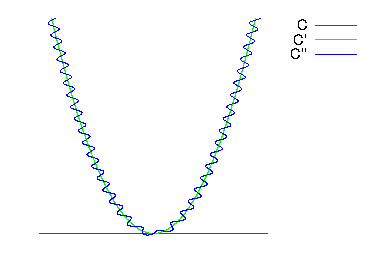
\includegraphics{x_squared_colour.pdf}
 \caption{An example for transformations.
   $\C$ represents a co-ordinate axis which is then transformed into a
 parabola, $\C^\prime$.  Finally a sinusoid is set about this
 $\C^\prime$ which give  $\C^\dprime$.
 Determining this function is a nice toy example to demostrate the
 power of geometric calculus.
}
 \label{fig:example_plots}
\end{figure}
Let us put these techniques to use in a simple example.
We begin with a curve embedded in a two dimensional Euclidean space,
and denote this curve $\C$.
%This curve will take the role of the `x-axis' in this discussion.
We then transform this into a second curve $\C^\prime$,
drawn so that $\C^\prime$ is a parabola with respect to $\C$.
%In the two dimensional space we are considering, 
When $\C$ is a straight line that takes a role of the `x-axis',
the curve $\C^\prime$ corresponds to the graph `$x^\prime = f(x) = x^2$'.
%, the axis with respect to which we are drawing the transformation.
We continue by drawing a third curve $\C^\dprime$,
which is a sinusoidal variation of $\C^\prime$. 
That is, we wish to draw the graph `$f^\prime(x^\prime) = \epsilon \sin(\abs{x^\prime})$' where
$\epsilon$ is a constant and $\abs{x^\prime}$ is the distance along
the curve $C^\prime$.
This example  will help to demonstrate how geometric calculus can be used to simply
solve problems that are far from trivial using coordinate methods.
The curves are drawn in \figref{example_plots}.  
It is our task to explicitally calculate their parameterisation.





% We consider a simple example.
% We wish to plot the two graphs of \figref{example_plots}.
% The first of these is the curve $\C^\prime := y^\prime = x^2$,
% while the second, $\C^\dprime$,  plots a sinusoidal variation about $y^\prime$.
% That is the sinusoid follows the bend in $y^\prime$.

% Implicit in the definition of $\C^\prime$ is an underlying coordinate basis,
% namely a Euclidean basis 
% \eql{
% {\gamma_i} = \{\gg, \ggg\}
% }{Euclidean_basis}
%  where
% $\gamma_i \cdot \gamma_j = 1$ if $i=j$ and $0$ otherwise.
% Then $y^\prime$ is the coordinate along the $\ggg$ axis,
% and $x$ is the coordinate along the $\gg$ axis.
% For curve $C^\prime$ such a basis enables the function to be expressed very
% simply.
% To represent $C^\dprime$ in such a basis is less convenient.

% Geometric algebra helps even in this simple example by letting much of
% the analysis to be done in a coordinate free manner.
% Then at the end,
% for the purposes of plotting the graph,
% we can introduce a convenient basis.







% Our graph can be expressed as a set of curves ${\C_i}$ embedded within a
% Euclidean two dimensional space spanned by the pseudoscalar $i$.
% For the purposes of drawing a graph we need a reference curve, $C$, 
% that takes the role of the `x-axis' in co-ordinate methods.

% Each of the curves are represented by a path
% \eq{
%   \C := x(\lambda) 
% }
% where $x$ is a vector intrinsic to the embedding space.
% Each of the curves can be considered as 1-dimensional vector manifolds
% within the 2-dimensional embedding space.
% If $p$ and $q$ are two points on the curve $\C_i$ then
% the vector $q-p$ is a chord of $\C_i$ from $p$ to $q$.
% In the limit the chords define a tangent vector to the curve so
% that  vector $a(x)$ is a tangent to a curve $\C$ at the point $x$ if
% \eq{
% a(x) = a\cdot \d x \equiv \left.\frac{dx(\lambda)}{\d \lambda}\right|_{\lambda =0}
% = \lim_{\lambda\rightarrow 0} \frac{x(\lambda) - x}{\lambda}.
% }
% The path can be reparameterised by the lengths of its cords,
% $\tau(\lambda) \equiv \abs{x(\lambda) - x}$,
% so that
% \eq{
% a = \frac{d\tau}{d\lambda} \frac{dx}{d\tau}.
% }
% The magnitude and unit direction of the tangent can then be identified
% as
% \eqal{
% \abs{a} = \frac{d\tau}{d\lambda} &,& \hat{a} = \frac{dx}{d\tau} = \frac{dx}{\abs{dx}},
% }{tangent_magnitude_and_unit}
% respectively.
% The unit tangent
% \eqa{
% v =\hat a =  \frac{dx}{d\tau} &,& v^2 = 1,
% }
% is known as the {\em velocity} of the curve.

% The parameter $\tau$ is unique to the curve in that we can identify $d\tau =\abs{dx}$.
% It follows that we can define a parameterisation-independant
% interval $(d\tau)^2 = dx\cdot dx$,
% which upon reintroducing an arbitrary parameterisation gives
% \eqal{
%  \left(\frac{d\tau}{\lambda}\right)^2 = \frac{dx}{d\lambda}\cdot\frac{dx}{d\lambda}.
% }{differential_length}
% The length of an arc on the path can be then be found to be
% \eql{
% \Delta \tau = \int_{\lambda^\prime}^{\lambda^\dprime}\left(\frac{dx}{d\lambda}\cdot\frac{dx}{d\lambda}\right)^{\half}d\lambda,
% }{defn_length}
% which is again invariant to a reparametrisaton.


When we draw a graph we follow the `independent-axis' to a given point,
and then leave that axis in the orthonal direction a distance determined
by some function, $\beta(x)$.
So by representing the independent-axis as a manifold (for example, the curve
$\C$ in the 2-dimensional case),
the map to the second manifold  is represented
\eql{
f: a \rightarrow a^\prime = f(x) = x + \beta(x) n(x),
}{graph_function}
where $x$ points to a point on the  manifold, and $n(x)$ is a vector entirely extrinsic (normal)
to the manifold at $x$. % so that $x\codt n = 0$.
The normal vector is defined to be the dual of the local-pseudoscalar on
the manifold, $I(x)$, such that
\eql{
  I(x) = n(x)i.
}{normal_definition}
The transformation of \eqnref{graph_function} is considered for arbitrary multivectors in
arbitrary dimensions by
\cite{Hestenes1984}.
Howerver, for our perposes the soley vectorial scope of
\eqnref{graph_function} are sufficient.
Since the pseudo-scalar to a curve is its velocity \eqnref{normal_definition}
reduces to
\eq{
  n(x) = v(x) i.}


Writing the transformation we seek is then easy,
\eqa{
  x^\prime = f(x) = x + \beta(x) v(x)i &,& \beta(x) &= x^2, \label{eqn:beta_zero}\\
  x^\dprime = f^\prime(x^\prime) = x^\prime + \beta^\prime(x^\prime) v^\prime(x^\prime)i &,& \beta^\prime(x^\prime) &= \sin(2\pi\omega\Delta\tau), \label{eqn:beta_one}
}
where $\Delta \tau$ is evaluated for position $x^\prime$ using \eqnref{defn_length}.

To plot \eqnref{beta_one} the velocity $v^\prime$ of $\C^\prime$ is
requred.
To obtain the tangent vectors to $\C^\prime$ from the tangent vectors
of $\C$ the  directional derivative,
$\fbar(a)= a\cdot\d f(x)$, is required.
Applying this to \eqnref{beta_zero} while remembering that $\d_x$ is the differential intrinsic to the curve $C$,
and so leaves alone the vector $n(x)$, gives
\eq{
 \fbar(a) = a + 2a\cdot x n. %\\
% \fbar^\prime(a^\prime) &= a^\prime + 2\pi\omega \cos(2\pi\omega\Delta \tau)\d\Delta \tau.
}
Remembering that the velocity is a curve's pseudoscalar and using
\eqnref{Jacobian} we obtain
% \eq{
% \fbar(v) = J_f v^\prime.
% }
% This can also be seen through use of the chain rule
% \eq{
% v^\prime(x^\prime) = \frac{dx^\prime}{d\tau^\prime} =
% \frac{d\tau}{d\tau^\prime}\frac{dx}{d\tau} \cdot\d f  = \frac{1}{J_f}\fbar(v). %&,&v^\dprime(x^\dprime) = \fbar_2(v^\prime),
% }
% So 
\eqa{
\fbar(v) &= v + 2 v\cdot x n = J_f v^\prime. \label{eqn:ExFbar}\\
\intertext{Upon squaring this leaves}
\left(\fbar(v)\right)^2 &= 1 + 4 \left(v\cdot x\right)^2 = J_f^2,\\
\intertext{and so the Jacobian of the transformation is given by}
 J_f &= \sqrt{ 1 + 4 \left(v\cdot x\right)^2 }. \label{eqn:ExJacobian}
}

Although it is not needed in this example it is worthwhile explicitly
calculating the adjoint function,
% The function
% \eq{
%  a^\prime = \fbar(a) =  a\cdot \del_x f(x)
% }
% maps the tangent vector $a(x)$ to the curve $C$ at the point $x$ to the
% tangent vector $a^\prime(x\prime)$ to the curve $C^\prime$ at the point
% $x^\prime$.
% Note that $\del_x$ is the differential intrinsic to the curve $C$,
% and so leaves alone the vector $n(x)$.
% Therefore we can write
% \eq{
% v^\prime(x^\prime) = \frac{dx^\prime}{d\tau} = \frac{dx}{d\tau} \cdot\d f  =\fbar(v). %&,&v^\dprime(x^\dprime) = \fbar_2(v^\prime),
% }
% Applying to \eqnref{beta_zero} and \eqnref{beta_one} gives
% \eq{
%  \fbar(a) = a + 2a\cdot x n, %\\
% % \fbar^\prime(a^\prime) &= a^\prime + 2\pi\omega \cos(2\pi\omega\Delta \tau)\d\Delta \tau.
% }
%Using
\eqa{
\fadj(a^\prime)& = \d_a \fbar(a) \cdot a^\prime \\
 &= \d_a  \left( a + 2a\cdot x n\right) \cdot a^\prime\\
 &= P(a^\prime + 2x n\cdot a^\prime),
}
where we are projecting onto $\C$.
Then
\eqa{
  \fadj\fbar(v) &= P\left( v + 2 v\cdot x n  + 2x n\cdot \left( v + 2 v\cdot x n \right)\right)\\
&= P\left( v + 2 v\cdot x n + 4x v\cdot x \right) v v \\
&= \left(  1 +  4 (v\cdot x)^2 \right) v \\
&= J_f^2 v,
}
as expected.

To actually plot the graphs we need to define a coordinate system for
the embedding space.
Using the Euclidean space defined in \eqnref{Euclidean_basis}
we may define the pseodoscalar of the 2-dimensional space as
\eq{
 i = \gg\ggg.
}
Setting the origin to be on the curve $C$ we choose
$v(x) = \gg$.
This implies that $n(x) = \gg i = \ggg$.
That is, the curve 
\eql
{
 \C : x(\tau) = \tau \gg
}{C_defn}
 is the `x-axis' for our graph,
and the normal is the `y-axis'.

Subsitutiong \eqnref{C_defn} into \eqnref{ExJacobian}
gives
\eqa{
  J_f &=  \sqrt{ 1 + 4\tau^2 }\\
\intertext{and so}
v^\prime &= \frac{\gg + 2\tau \ggg}{\sqrt{ 1 + 4\tau^2 }},
\intertext{where \eqnref{ExFbar} has been used.
Calculating $n^\prime$   with \eqnref{tau_primed} gives:}
 n^\prime = v^\prime i &=\frac{\ggg - 2 \tau\gg}{\sqrt{1+4\tau^2}}.
}
% where \eqnref{ExFbar} has been used.
% Calculating $n^\prime$  explicitly:
% \eql{
%   n^\prime = v^\prime i =\frac{\ggg - 2 \tau\gg}{\sqrt{1+4\tau^2}},
% }{n_primed}
% where we have used \eqnref{tau_primed}
% Next we define a basis for the curve $\C^\prime$,
% \eq{
%   e_i \equiv \fbar(\gamma_i)
% }
% and find
% \eqa{
%   e_1(\tau) = v^\prime(\tau) =J_f v^\prime(\tau^\prime) = \gg + 2\tau \ggg &,&e_2 \ne n^\prime =  \ggg.
% }
% Writing 
% \eq{
% v^\prime(\tau^\prime) = \frac{dx^\prime}{d\tau^\prime} =
% \frac{d\tau}{d\tau^\prime}\frac{dx^\prime}{d\tau} =
% \frac{d\tau}{d\tau^\prime}v^\prime(\tau) = 
% J_f v^\prime(\tau)
% }
% and enforcing $v^{\prime 2}(\tau^\prime) = 1$ gives
% \eq{
% v^\prime(\tau^\prime) = \frac{v^\prime(\tau)}{\sqrt{1+4\tau^2}}.
% } 
% %Writing $\tau^\prime = \epsilon \tau$ gives
% %\eq{
% %  v^\prime(\tau^\prime) = \epsilon \gg + 2\epsilon\tau\ggg,
% %}
% %and enforcing $v^{\prime 2} = 1$ implies that
% %\eql{
% % \tau^\prime = \frac{\tau}{\sqrt{1+4\tau^2}}.
% %}{tau_primed}
% Calculating $n^\prime$  explicitly:
% \eql{
%   n^\prime = v^\prime i =\frac{\ggg - 2 \tau\gg}{\sqrt{1+4\tau^2}},
% }{n_primed}
% where we have used \eqnref{tau_primed}
All that is required now is to find $\delta \tau$ between the origin and
$x^\prime$,
\eqa{
\Delta \tau &= \int_0^{\tau_\text{max}} \sqrt{ \fbar(v)\cdot \fbar(v)}d\tau 
 = \int_0^{\tau_\text{max}} \sqrt{1 + 4\tau^2  } d\tau\\
 &= \frac{1}{4} \left[
    \ln\left( 2\tau_\text{max} + \sqrt{1 + 4\tau_\text{max}^2 } \right) + 2\tau_\text{max} \sqrt{1 + 4\tau_\text{max}^2  }
\right] \label{eqn:example_delta_time}\\
&= \frac{1}{4} \left[ \ln\left( 2\tau_\text{max} + J_f \right) + 2\tau_\text{max} J_f \right]
}
where the standard identity $\cosh\sinh^{-1}(x) \equiv \sqrt{1+x^2}$ has
been used to put the integral in the form of \eqnref{example_delta_time}.

Pulling this together with the help of \eqnref{beta_zero} and \eqnref{n_primed},  we find
\eqa{
\C: x(\tau) &= \tau \gg\\
  \C^\prime: x^\prime(\tau) &= \tau \gg + \tau^2 \ggg \\ 
\C^\dprime: x^\dprime(\tau) &=  \tau \gg + \tau^2 \ggg  +
\epsilon J_f^{-1}\sin(2\pi\omega\Delta\tau) \left(\ggg - 2 \tau\gg\right)\nonumber \\
  &= \left(\tau - 2\tau\epsilon J_f^{-1}\sin(2\pi\omega\Delta\tau)
  \right) \gg 
    + \left(\tau^2 + \epsilon J_f^{-1}\sin(2\pi\omega\Delta\tau) \right) \ggg,
}
which is what is drawn in \figref{example_plots}.

Note that this example was straightforward using geometric algebra.
The interpretation of the quantities that were being evaluated at each
stage was clear, and by choosing a co-ordinate system at the end,
after the transformations had beed identified, the actual calculations
were short.
This would not have been the case for standard coordinate methods.
For instance, standard differential geometry does not keep track of
the extrinsic geometry to a manifold, and so our use of the normal
vector would require the introduction of a `fibre bundle',
with all the book-keeping that this would entail.




% As a first step we must invert
% \eq{
%   x^\prime(\tau) = \tau \gg + \tau^2 \ggg
% }
% The inequality of $e_2$ with $n^\prime$ is required so that the space


% To find the 
% The velocity of $\C^\prime$ is equal to the 

% We need a transformation to map between the curves
% A graph is simply a surface representing the height 

%   `dependent-variable' plotted
% orthogonally to a set of 
% 'independant-variables'.
% This can be achieved geometrically by transforming the surfance
% representing the indpedent variables into by reprenting each curve by a manifold.

% plotting a dependent-manifold
% tranformed ind
% representing the indepedent
% variables with a manifold which is transformed in the direction of a
% normal vector that is entirely extrinsic to the manifold.


% the manifold (in this case a curve) to represent the indepedent
% varibles we can define a normal vector $n$ that is entirely extrinsic to
% the manifold.
% In this case the normal vector at a position $x_\mu$ on curve $\C_\mu$ is
% \eq{
% n_\mu(x_\mu) = v(x_\mu) i.
% }



% A point in a graph should relate to its various axes via a projection.
% That is 
% a point $x_1(\tau_1)$ on $\C_1$ should map to the point $x(\tau)$ on $\C$
% by projection.
% That is
% \eq{
% f_1^{-1}: x_1 \rightarrow x = f_1^{-1}(x_1) = P(x_1)
% }

% where $P_{\C}(\cdot)$ reprents a projection operation onto the curve $C$.
% The appropriate projection operator is


% To map from $\C\rightarrow\C_1$ we should move along the curve $\C$
% to a position $x$,
% then we should 

% saying that
% the `dependent-variable' should sit  should
% and we can include this is a co
% For drawing a graph the notion of orthogonality between 
% The notion of othogonality between 
% Let us consider the transformation between the curves
% \eq{
%  f(x) = x + \beta(x) xi.
% }
% This function 


% with respect to which the curve $\C_1$ will be
% drawn, $\C$ takes the role of the `x-axis' in co-ordinate methods.


% The curve $C_1$ is then a mapped from $C$ via the transformation
% \eq{
%  C
% }

%  of two functions.
% Firstly, 
%  simple function $\beta(x) = x^2)$ with respect to a



%  of where we want to plot a 
% \eqa{
% x^\prime &= f(x) = x + \beta(x)n\\
% x^{\dprime}&= g(x^\prime) = g(f(x))  = x^\prime + \beta^\prime(x^\prime) n^\prime
% }
% where
% \eqa{
% x &= \lambda e_1\\
% n &= \hat x i \\
% n^\prime &= \hat \fbar(x) i \\
% i &= e_1 e_2
% }
% where for the purpose of the example 
% \eqa{
% \beta(x) &= x^2 \\
% \beta^\prime(x^\prime) &= \sin(x^\prime\cdot\fbar(e_1))
% }
% so that
% \eqa{
% a \cdot \d_x x^\prime = \fbar(a) &= a + a\cdot \d_x \beta(x) n\\
% &= a + 2 a \cdot x n
% }
% and
% \eqa{
% a\cdot \d_{x^\prime}x^\dprime = \underbar{g}(a^\prime) &=
%   a^\prime + a^\prime \cdot \d_{x^\prime}
%   \beta^\prime(x^\prime)n^\prime\\ 
% &= a^\prime + a^\prime \cdot \cdot\fbar(e_1)  \cos(x^\prime\cdot\fbar(e_1))
% }
% So
% \eqa{
% x^\prime = f(\lambda e_1) &= \lambda e_1 + \lambda^2 e_2 \\
% \fbar(e_1; \lambda) &= e_1 + 2 \lambda e_2
% }
% setting $a^\prime = \fbar(e_1)$
% \eqa{
% g(x^\prime) &= x^\prime + \sin(x^\prime \cdot f(e_1)) n^\prime \\ \nonumber
% &=\left[\lambda(1 - \lambda\sin(\lambda(1+2\lambda^2)))\right]e_1 \\ 
% &+ \left[\lambda(\lambda + \sin(\lambda(1+2\lambda^2)))\right]e_2\\
% }
% and 
% \eqa{
% \underbar g(\fbar(e_1)) &= 
% \fbar(e_1) + \fbar^2(e_1)\cos(\fbar^2(e_1)) \fbar(e_1)e_1e_2 \\ \nonumber
% &= \left[1 - 2\lambda(1+\lambda^2)\cos(1+\lambda^2)  \right]e_1 \\ &+
%    \left[2\lambda + (1 + 4\lambda^2)\cos(1+4\lambda^2)\right]e_2
% }

\subsection{Functional Derivative}
% The "bracket thing" is an inner product for functions (more generally distributions which are formal functions define only inside integrals and not necessarily in terms of values, as e.g. the Dirac delta "function")

% But there is a problem with your invocation of the chain rule. The functional $\mathcal{F}$ maps functions to scalars. If you assume $\rho$ is again a functional then you can't compose it with $\mathcal{F}$

% In general you can't compose functionals since their domain and range are distinct types (functions vs numbers).

% So you can either have a chain rule of the form:
% \eq{
% \frac{\delta\mathcal{F}[\rho(\sigma)]}{\delta \sigma}= \frac{\delta \mathcal{F}[\rho]}{\delta \rho}\frac{d \rho}{d \sigma}
% }
% Or invoke a parameterized functional (functional valued function) which will give a much messier chain rule.

% It may help (though not I think to prove the general case) to start
% with functionals defined by integrals, i.e.:
% \eq{
% \mathcal{F}[\rho] \equiv \int \phi(\rho(x))dx
% }
% then you get functional differential:
% \eq{
% \delta \mathcal{F}[\rho] = \int \frac{d \phi(\rho)}{d\rho}\delta \rho dx
% }
% Then the functional derivative (as a distribution) is:
% \eqa{
% \left\langle \frac{\delta \mathcal{F}[\rho]}{\delta\rho} , f\right\rangle=\int\frac{d \phi(\rho)}{d\rho} f dx
% \intertext{thence}
% \frac{\delta \mathcal{F}[\rho]}{\delta\rho} =\frac{d \phi(\rho)}{d\rho}= \phi' \circ \rho
% }
% In standard calculus you will note that the derivative of a function is a multiplier for a linear term in the variable. The n-th derivative is the multiplier for an n-th degree term. Effectively then the first derivative times the variable is a linear function, and higher order n-th degree functions.

% In the functional case, the first functional derivative contracts with
% the variable (a function) to yield a linear functional. This is why
% you get a "distribution" instead of a function. Because the space of
% functions is infinite dimensional, its dual space consists of more
% than linear functionals of the form:
% \eq{
% f \mapsto \left\langle \phi , f \right\rangle
% }
% where $\phi$ is a function. We must define a more general class of objects, distributions which are only defined by first giving a linear functional and then rewriting it in the form of an inner product above but with the $\phi$ not meaningful as an actual function.

% Note you can generalize further by considering an operator (not necessarily linear) which maps functions to functions and for which we can (with some restrictions) define an operator derivative
% \eq{
% \frac{\Delta \Omega[\phi]}{\Delta \phi}
% }
% as an linear operator (for a given $\phi$).

% Thence:
% \eq{
% \frac{\Delta \Omega[\phi]}{\Delta \phi}[a \xi + b \eta] =a\frac{\Delta \Omega[\phi]}{\Delta \phi}[\xi] +b\frac{\Delta \Omega[\phi]}{\Delta \phi}[\eta]
% }
% is a function. (a and b scalars, f and g functions.)

% Since you can compose operators you can then better discuss an operator chain rule:
% \eq{
% \frac{\Delta \Omega[\Xi[\psi]]}{\Delta \psi}[f] = \frac{\Delta \Omega[\Xi[\psi]]}{\Delta \Xi}\left[\frac{\Delta \Xi}{\Delta \psi}[f]\right]
% }
% In essence one generalizes the Taylor expansion of a general operator
% in terms of "constant" plus linear operator plus bilinear operator ...



% I noticed that I didn't actually give you the definition of the operator derivative. It is defined as a linear operator such that for small variations of the function:
% \eq{
% \Omega[f+\delta f] = \Omega[f]+ \frac{\Delta\Omega[f]}{\Delta f}[\delta f] + O(\delta f^2)
% }

% To get more rigorous:
% \eq{
% \Omega[f+\delta f](x) = \Omega[f](x)+ \frac{\Delta\Omega[f]}{\Delta f}[\delta f](x) + O(\delta f^2)
% }
% where the order of the square of the variation is defined by taking the maximum magnitude of $\delta f(x)\cdot \delta f(y)$ for all values of x and y.

% You can then define the derivative explicitly by:
% \eqa{
% \frac{\Delta\Omega[f]}{\Delta f}[\delta f](x) = \lim_{\epsilon\to 0}\\
% \frac{\Omega[f + \epsilon\delta f](x)-\Omega[f](x)}{\epsilon}
% }
% where $\delta f$ is any of a restricted class of functions e.g. test functions or bounded smooth functions with compact support or something similar.

% Here is a clarifying example.

% The derivative of a function is the action of an operator $\mathbf{D}$ on that function.

% We can thus take the operator derivative of the differential operator:
% \eq{
% \mathbf{D}'[f] = \frac{\Delta \mathbf{D}[f]}{\Delta f}
% }
% Since we are taking an operator derivative $mathbf{D}'[f]$ will be a linear operator. But since the derivative is a linear operator its derivative will be a constant (with regard to f).

% In short $\mathbf{D}'[f_1] = \mathbf{D}'[f_2]$.

% So the "value" of the "derivative of the derivative" is:
% \eq{
% \mathbf{D}'[f][g]= \lim_{\epsilon\to 0}\frac{\mathbf{D}[f+\epsilon g]-\mathbf{D}[f]}{\epsilon}
% =\lim_{\epsilon\to 0} \frac{\mathbf{D}[f] +\epsilon\mathbf{D}[g]-\mathbf{D}[f]}{\epsilon} = \mathbf{D}[g]
% }
% So the "derivative of the derivative" is "the derivative" in the same sense that the derivative of f(x)=cx is c viewed as a linear multiplier.

% It may help more to think of the operator derivative as acting like a Greens function:
% The derivative being linear can be expressed as an integral:
% \eq{
% \mathbf{D}[f](x) = \int \delta'(x-y)f(y)dy
% }
% where $\delta'(x-y)$ is the formal derivative of the Dirac delta function (limit of derivatives of normalized Gaussian functions as the variation goes to zero).


% The derivative then is the linear operator defined in "component form" by the two valued function $D(x,y) = \delta'(x-y)$. Think of the variables as acting analogous to the indices of vectors or matrices.

% You can think of the higher order functional and operator derivatives as generalized Taylor expansions:

% For functionals:
% \eq{
% \mathcal{F}[\phi] = F^{(0)}+ \int F^{(1)}(x)\phi(x)dx + \iint F^{(2)}(x,y)\phi(x)\phi(y) dx dy + \iiint F^{(3)}(x,y,z)\phi(x)\phi(y)\phi(z)dx dy dz + \cdots
% }
% For operators:
% \eq{
% \Omega[\phi](x) = \Omega^{(0)}(x) + \int \Omega^{(1)}(x,y)\phi(y)dy + \iint \Omega^{(2)}(x,y,z)\phi(y)\phi(z) dy dz + \cdots
% }
% where these "multi-variable functions" $\Omega^{(k)}$ are rather multi-distributions since they only appear in integrals.



The functional $F[\genf]$ is to be minimised,
that is, we wish to find the function $\genf$ that remains invarient
under the transformation $\genf \rightarrow \genf + \epsilon g$, where
$\epsilon$ is a small constant and $g$ is an arbitrary function.



From \cite{Lasenby1993} we have:

Want to evaluate
\eq{
  \d_{\fbar(b)} \fbar(A_r)
}
where
\eq{
 \fbar(b) = b\cdot \del f(x)
}
and so assume that we evaluate differential at the same point $x$.

First project $A_r$ onto the vector $b$,
\eq{
 P_b (A_r) = (A_r\cdot b^{-1}) b = b\wedge(b^{-1}\cdot A_r),
}


It can be conceptually useful to discretise the input to the function
into an
%
%the function $\genf$ into an
%$N$ dimensional vector, paramameterised by the 
$N$ dimensional Cartesian
basis $e_n$, $n = 1, 2, \ldots, N$:
\begin{align}
& \genf \rightarrow \genf_j  \equiv \genf(e_j), &g \rightarrow g_k  \equiv g(e_k) &
\end{align}
The components of the vector can be found by contracting with the basis,
\begin{align}
 g_{ik} \equiv  e_i \cdot g_k
\end{align}

%where $\genf_j$ is the $j^{th}$ component of the vectorised function
%$\genf$.
The continuum limit can be recovered later by letting
$N\rightarrow\infty$.



A set of $N$ directional derivaties can then be evaluated in the usual
way,
\begin{align}
 g_k \cdot \d_{\genf_j} F( \genf_j ) &= \lim_{\epsilon \rightarrow 0} \frac{1}{\epsilon}
   \left( F( \genf_j + \epsilon g_k)  - F( \genf_j )  \right)
\\
e_i \cdot \d_{\genf_j} F( \genf_j ) g_{ik} &=\lim_{\epsilon \rightarrow 0} \frac{1}{\epsilon}
   \left( F( \genf_j + \epsilon e_i)  - F( \genf_j )  \right)g_{ik},
\end{align}
where we are summing over the repeated index $i$.
The derivative over the discretised function $f$ is then the sum over
these $N$ directional derivatives,
\begin{align}
 dF &=  \sum_k^N g_k \cdot \d_{\genf_j} F(\genf_j) 
 \label{eqn:vectorized_functional_derivative}
\end{align}
The right hand side can be simplified by making the following
definition,
\begin{align}
e_i \cdot \d_{\genf_j} = \d_{e_i \cdot \genf_j} \equiv \d_{\genf_{ij}},
\end{align}
so that \eqnref{vectorized_functional_derivative} can be written
\begin{align}
 dF &=  \sum_{k}^N \d_{\genf_{ij}} F(\genf_j) g_{ik}.
\end{align}

From \cite{Doran2003},
\begin{align}
 f_{ij} = e_i \cdot \genf(e_j).
 \end{align}
so that
\begin{align}
 \d_{f_{ij}} \genf(b)\cdot c &= \d_{f_ij} (\genf_{lk} b^k c^l) \\
 &= c^i b^j
\end{align}
So mulitplying by $a\cdot e_j e_i$ we get
\begin{align}
 a\cdot e_j e_i \d{\genf_{ij}} \genf(b)\cdot = a \cdot b c,
\end{align}

so
\begin{align}
 \d_{\genf(a)} = a\cdot e_j e_i \d_{f_{if}}
\end{align}
so that 
\begin{align}
 \d_{\genf(a)} \genf(b)\cdot c = a\cdot b c
\end{align}

In general we have
\begin{align}
  \d _{\genf(a)} \scalar{\genf(A)B} = \sum_r \mono{\genf(a\cdot A_r)B_r}
\end{align}
so that for a fixed grade multivector we can write
\begin{align}
 \d_{\genf(a)} \genf({A_r}) = \left(n-r+1\right)\genf(a\cdot A_r)
\end{align}

Use in the Euler Lagrange Equations:
\begin{align}
\frac{\d}{\d\genf(e^j)} &= e_i \frac{\d}{\d \genf_{ij}}
\end{align}

If
\begin{align}
\genf(a) = a\cdot \d f(x) 
\end{align}
then
\eq{
  \genf_{ij} = e_i \cdot \genf(e_j) = e_j \cdot (\d_i f)
}
so that
\eq{
\frac{\d}{\d(\d_j f)} = e_j \frac{\d}{\d_{\genf_{ij}}}= \frac{\d}{\d\genf(e^j)}
}


%\section{Lagrangian Mechanics}




Mostly taken from \cite{Lasenby1993}.
The scalar valued function 
\eq{
L = L(\psi_i, \dot{\psi}_i),
}
where $\psi_i$ are a set of general multivectors.

Extremise the action
\eq{
S = \int_{t_i}^{t_f} dt L(\psi_i, \dot{\psi}_i)
}
with respect to $\psi_i$.
We write 
\eq{
 \psi_i(t) = \psi_i^0(t) + \epsilon \phi_i(t)
}
where $\phi_i$is a multivector of the same grades as $\psi_i$,
$\epsilon$ is a scalar and $\psi_i^0$ represents the extremal path.

Take the derivative wrt $\epsilon$ to get
\begin{align}
  \d_\epsilon L &= \int_{t_i}^{t_f} dt \left( 
    \phi_i \ast \d_{\psi_i} L + \dot{\phi}_i\ast \d_{\dot{\psi}_i} L
    \right)\\
&= \int_{t_i}^{t_f} dt  
    \phi_i \ast \left(\d_{\psi_i} L - \d_t( \d_{\dot{\psi}_i} L) \right)
+
\left[ \phi_i\ast\d_{\dot{\psi}_i } L  \right]_{t = t_i}^{t = t_f}
\end{align}
For stationarity this must vanish for all $\phi_i$,
giving the Euler-Lagrange Equations
\eq{
\d_{\psi_i} L - \d_t(\d_{\psidot_i}L) = 0
}

\subsection{Transformation}
Consider transformation parameterised by a single multivector $M$
\eq{
 \psi_i^\prime = f(\psi_i, M)
}
where $f$ and $M$ are time independent.

Define:
\eq{
  \fbar_A(\psi_i, M) = A\ast \d_M f(\psi_i, M)
}
and
\eq{
L^\prime = L(\psi_i^\prime, \psidot_i^\prime)
}
gives
\begin{align}
A\ast\d_M L^\prime &=
 \fbar_A(\psi_i, M) \ast \d_{\psi_i^\prime} L^\prime + 
 \fbar_A(\psidot_i, M) \ast \d_{\psidot_i^\prime}L^\prime
\\
&= \fbar_A(\psi_i, M)\ast\left(\d_{\psi_i^\prime} L^\prime -
 \d_t(\d_{\psidot_i^\prime} L^\prime)\right)
+ \d_t\left(\fbar_A(\psi_i, M) \ast \d_{\psidot_i^\prime}L^\prime\right)
\end{align}
Assuming that the equations of motion are satisfied by $\psi_i^\prime$
gives
\begin{align}
A\ast\d_M L^\prime = \d_t\left(\fbar_A(\psi_i, M) \ast
 \d_{\psidot_i^\prime} L\right)
\end{align}
Differentate out the $A$ dependance
\begin{align}
 \d_M L^\prime &= \d_t \left( \d_A \fbar_A (\psi_i, M) \ast \d_{\psidot_i^\prime}L^\prime\right)
&= \d_t\left(\rd_M \psi_i^\prime \ast \d_{\psidot_i^\prime}L^\prime\right)
\end{align}

If $L^\prime$ is independent of M then
 $\d_A \fbar_A(\psi_i, M)\ast\d_{\psidot_i^\prime}L^\prime$ is
 conservered.

If $M$ is a scalar parameter, $\alpha$ then
\begin{align}
 \d_\alpha L^\prime = \d_t \left( (\d_\alpha \psi_i^\prime)\ast \d_{\psidot_i^\prime}L^\prime \right)
\end{align}
e.g.
\begin{align}
\psi_i^\prime(t,\alpha) &= \psi(t+\alpha)\\
\text{gives } \given{\d_\alpha \psi_i^\prime}{\alpha = 0} &= \psidot_i
\end{align}

If all $t$-dependance enters $L$ through the dynamical variables only we
get
\begin{align}
\d_t L = \d_t \left(\psidot_i \ast \d_{\psidot_i} L\right)
\end{align}
and the conserved Hamiltonian as
\begin{align}
 H = \psidot_i \ast \d_{\psidot_i}L - L
\end{align}

%\section{Field Theory}

The introduction of symmetry arguments is most easily accomplished
with field theory.
Additionally, the writing of dynamics into a single lagragnian means
that a self consistent set of contraints has been provided,
and in this sence makes a good check.

So we write a scalar lagragian $\L$ according to the zeroth and first
derivatives of a set of  multivector fields $\psi_i(x)$,
\eq{
\L = \L(\psi_i, \del \psi_i).
}
We wish to minimise the action
\eq{
S = \int\abs{d^4x}\L.
}
with respect to $\psi_i$ and so we write 
\eq{
\psi_i(x) = \psi_i^0(x) + \epsilon \phi(x),
}
where $\psi_i^0(x)$ is the minimal field.

To minimise we take the derivative with respect to $\epsilon$
\eq{
\d_\epsilon S = \int \abs{d^4x} \left(\phi\star\d_{\phi_i} \L + (\del
  \phi_i)\star \d_{\del \psi_i} \L\right).
}
The last term can be written
\eq{
 \scalar{\dot \del \dot \phi_i \d_{\del \psi_i} \L } = 
  \del\cdot\scalar{\phi_i \d_{\del \psi_i}\L} - \phi_i \star 
\left( (\d_{\del \psi_i} \L) \ldel \right)
}
assuming boundary vanish get
\eq{
 \d_\epsilon S = \int \abs{d^4x}\psi\star
\left(\d_{\psi_i}\L - (\d_{\del \psi_i} \L ) \ldel \right)
}
If $\psi_i$ contains only terms of grade-$r$ then the appropriate
Euler-Lagrange equations are
\eq{
\multi{\d_{\psi_i}\L - (\d_{\del \psi_i} \L) \ldel}{r} = 0,
}
wheras if $\psi$ is a general even multivector then
\eq{
\d_\psi \L = (\d_{\del \psi}\L) \rdel
}
%
%
%\section{Functional Differentiation}
%
%From \cite{Lasenby1993} we have:
%
%Want to evaluate
%\eq{
%  \d_{\fbar(b)} \fbar(A_r)
%}
%where
%\eq{
% \fbar(b) = b\cdot \del f(x)
%}
%and so assume that we evaluate differential at the same point $x$.
%
%First project $A_r$ onto the vector $b$,
%\eq{
% P_b (A_r) = (A_r\cdot b^{-1}) b = b\wedge(b^{-1}\cdot A_r),
%}
%
%
%
%The functional $F[\genf]$ is to be minimised,
%that is, we wish to find the function $\genf$ that remains invarient
%under the transformation $\genf \rightarrow \genf + \epsilon g$, where
%$\epsilon$ is a small constant and $g$ is an arbitrary function.
%
%It can be conceptually useful to discretise the input to the function
%into an
%%
%%the function $\genf$ into an
%%$N$ dimensional vector, paramameterised by the 
%$N$ dimensional Cartesian
%basis $e_n$, $n = 1, 2, \ldots, N$:
%\begin{align}
%& \genf \rightarrow \genf_j  \equiv \genf(e_j), &g \rightarrow g_k  \equiv g(e_k) &
%\end{align}
%The components of the vector can be found by contracting with the basis,
%\begin{align}
% g_{ik} \equiv  e_i \cdot g_k
%\end{align}
%
%%where $\genf_j$ is the $j^{th}$ component of the vectorised function
%%$\genf$.
%The continuum limit can be recovered later by letting
%$N\rightarrow\infty$.
%
%
%
%A set of $N$ directional derivaties can then be evaluated in the usual
%way,
%\begin{align}
% g_k \cdot \d_{\genf_j} F( \genf_j ) &= \lim_{\epsilon \rightarrow 0} \frac{1}{\epsilon}
%   \left( F( \genf_j + \epsilon g_k)  - F( \genf_j )  \right)
%\\
%e_i \cdot \d_{\genf_j} F( \genf_j ) g_{ik} &=\lim_{\epsilon \rightarrow 0} \frac{1}{\epsilon}
%   \left( F( \genf_j + \epsilon e_i)  - F( \genf_j )  \right)g_{ik},
%\end{align}
%where we are summing over the repeated index $i$.
%The derivative over the discretised function $f$ is then the sum over
%these $N$ directional derivatives,
%\begin{align}
% dF &=  \sum_k^N g_k \cdot \d_{\genf_j} F(\genf_j) 
% \label{eqn:vectorized_functional_derivative}
%\end{align}
%The right hand side can be simplified by making the following
%definition,
%\begin{align}
%e_i \cdot \d_{\genf_j} = \d_{e_i \cdot \genf_j} \equiv \d_{\genf_{ij}},
%\end{align}
%so that \eqnref{vectorized_functional_derivative} can be written
%\begin{align}
% dF &=  \sum_{k}^N \d_{\genf_{ij}} F(\genf_j) g_{ik}.
%\end{align}
%
%From \cite{Doran2003},
%\begin{align}
% f_{ij} = e_i \cdot \genf(e_j).
% \end{align}
%so that
%\begin{align}
% \d_{f_{ij}} \genf(b)\cdot c &= \d_{f_ij} (\genf_{lk} b^k c^l) \\
% &= c^i b^j
%\end{align}
%So mulitplying by $a\cdot e_j e_i$ we get
%\begin{align}
% a\cdot e_j e_i \d{\genf_{ij}} \genf(b)\cdot = a \cdot b c,
%\end{align}
%
%so
%\begin{align}
% \d_{\genf(a)} = a\cdot e_j e_i \d_{f_{if}}
%\end{align}
%so that 
%\begin{align}
% \d_{\genf(a)} \genf(b)\cdot c = a\cdot b c
%\end{align}
%
%In general we have
%\begin{align}
%  \d _{\genf(a)} \scalar{\genf(A)B} = \sum_r \mono{\genf(a\cdot A_r)B_r}
%\end{align}
%so that for a fixed grade multivector we can write
%\begin{align}
% \d_{\genf(a)} \genf({A_r}) = \left(n-r+1\right)\genf(a\cdot A_r)
%\end{align}
%
%Use in the Euler Lagrange Equations:
%\begin{align}
%\frac{\d}{\d\genf(e^j)} &= e_i \frac{\d}{\d \genf_{ij}}
%\end{align}
%
%If
%\begin{align}
%\genf(a) = a\cdot \d f(x) 
%\end{align}
%then
%\eq{
%  \genf_{ij} = e_i \cdot \genf(e_j) = e_j \cdot (\d_i f)
%}
%so that
%\eq{
%\frac{\d}{\d(\d_j f)} = e_j \frac{\d}{\d_{\genf_{ij}}}= \frac{\d}{\d\genf(e^j)}
%}




%%% Local Variables: 
%%% mode: latex
%%% TeX-master: "tshorrock_thesis"
%%% End: 
